


\tikzset{every picture/.style={line width=0.75pt}} %set default line width to 0.75pt        

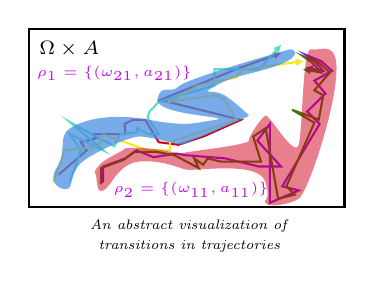
\begin{tikzpicture}[x=0.75pt,y=0.75pt,yscale=-1,xscale=1]
%uncomment if require: \path (0,1974); %set diagram left start at 0, and has height of 1974

%Shape: Rectangle [id:dp5335676631264512] 
\draw  [fill={rgb, 255:red, 255; green, 255; blue, 255 }  ,fill opacity=1 ] (190,1560.11) -- (342.1,1560.11) -- (342.1,1646) -- (190,1646) -- cycle ;
%Straight Lines [id:da6623576988919416] 
\draw [color={rgb, 255:red, 208; green, 2; blue, 27 }  ,draw opacity=1 ]   (308.67,1572.84) -- (290.28,1579.49) -- (253.26,1594.41) -- (292.1,1604) -- (274.1,1612) -- (262.1,1616) -- (252.58,1614.77) -- (246.1,1604) -- (240.1,1604) -- (236.1,1606) -- (236.51,1610.86) -- (220.44,1610.86) -- (223,1612.73) -- (215.09,1614.77) -- (217.85,1618.79) -- (204.38,1630.38) ;
\draw [shift={(311.49,1571.82)}, rotate = 160.12] [fill={rgb, 255:red, 208; green, 2; blue, 27 }  ,fill opacity=1 ][line width=0.08]  [draw opacity=0] (3.57,-1.72) -- (0,0) -- (3.57,1.72) -- cycle    ;
%Straight Lines [id:da5424854363807742] 
\draw [color={rgb, 255:red, 80; green, 227; blue, 194 }  ,draw opacity=1 ]   (309.47,1570.13) -- (300.78,1579.63) -- (279.36,1579.63) -- (279.36,1587.44) -- (252.58,1595.25) -- (250.1,1598) -- (248.1,1600) -- (247.22,1603.06) -- (252.58,1610.86) -- (247.22,1610.86) -- (242.1,1608) -- (242.1,1610) -- (233.94,1610.94) -- (231.16,1616.72) -- (209.73,1605.01) -- (225.8,1618.67) -- (209.73,1610.86) -- (215.09,1618.67) -- (209.73,1634.29) ;
\draw [shift={(311.49,1567.92)}, rotate = 132.45] [fill={rgb, 255:red, 80; green, 227; blue, 194 }  ,fill opacity=1 ][line width=0.08]  [draw opacity=0] (3.57,-1.72) -- (0,0) -- (3.57,1.72) -- cycle    ;
%Straight Lines [id:da21186841526109945] 
\draw [color={rgb, 255:red, 248; green, 231; blue, 28 }  ,draw opacity=1 ]   (319.23,1576.14) -- (292.83,1579.75) -- (290.07,1583.54) -- (271.41,1587.56) -- (257.93,1595.25) -- (280.1,1592) -- (284.1,1594) -- (290.1,1604) -- (257.93,1614.77) -- (257.93,1618.67) -- (247.22,1618.67) -- (225.99,1611.06) -- (223.21,1616.84) -- (207.14,1618.79) -- (201.78,1634.41) ;
\draw [shift={(322.2,1575.73)}, rotate = 172.2] [fill={rgb, 255:red, 248; green, 231; blue, 28 }  ,fill opacity=1 ][line width=0.08]  [draw opacity=0] (3.57,-1.72) -- (0,0) -- (3.57,1.72) -- cycle    ;
%Straight Lines [id:da6313290732282947] 
\draw [color={rgb, 255:red, 144; green, 19; blue, 254 }  ,draw opacity=1 ]   (326.23,1579.39) -- (331.84,1580.41) -- (327.56,1575.73) -- (323.27,1572.61) -- (330.86,1575.73) -- (336.13,1580.41) -- (327.56,1585.1) -- (332.91,1591.34) -- (324.1,1600) -- (330.1,1606) -- (312.1,1636) -- (320.1,1638) -- (306.1,1644) -- (306.1,1606) -- (300.1,1614) -- (311.49,1626.48) -- (300.78,1626.48) -- (294.99,1625.07) -- (291.92,1624.33) -- (287.57,1623.27) -- (284.71,1622.58) -- (273.96,1621.71) -- (265.43,1621.01) -- (261.23,1620.25) -- (250.1,1622) -- (241.87,1618.67) -- (236.51,1622.58) -- (225.8,1626.48) -- (225.8,1634.29) ;
\draw [shift={(323.27,1578.85)}, rotate = 10.33] [fill={rgb, 255:red, 144; green, 19; blue, 254 }  ,fill opacity=1 ][line width=0.08]  [draw opacity=0] (3.57,-1.72) -- (0,0) -- (3.57,1.72) -- cycle    ;
%Straight Lines [id:da1305524961942589] 
\draw [color={rgb, 255:red, 65; green, 117; blue, 5 }  ,draw opacity=1 ]   (325.15,1580.17) -- (330.77,1581.19) -- (326.49,1576.51) -- (322.2,1573.39) -- (329.79,1576.51) -- (335.06,1581.19) -- (327.56,1589.78) -- (331.84,1592.13) -- (329.7,1603.84) -- (316.85,1599.15) -- (327.56,1605.4) -- (314.1,1636) -- (318.1,1640) -- (310.1,1642) -- (304.1,1608) -- (298.1,1612) -- (301.85,1624.14) -- (289,1624.14) -- (282.57,1624.14) -- (276.14,1622.58) -- (274,1625.7) -- (269.72,1622.58) -- (271.86,1627.26) -- (260.16,1621.03) -- (251.51,1619.45) -- (240.8,1619.45) -- (235.44,1623.36) -- (224.73,1627.26) -- (224.73,1635.07) ;
\draw [shift={(322.2,1579.63)}, rotate = 10.33] [fill={rgb, 255:red, 65; green, 117; blue, 5 }  ,fill opacity=1 ][line width=0.08]  [draw opacity=0] (3.57,-1.72) -- (0,0) -- (3.57,1.72) -- cycle    ;
%Shape: Polygon Curved [id:ds29559681347985167] 
\draw  [color={rgb, 255:red, 184; green, 233; blue, 134 }  ,draw opacity=0 ][fill={rgb, 255:red, 74; green, 144; blue, 226 }  ,fill opacity=0.75 ] (203.31,1627.26) .. controls (208.88,1618.48) and (203.46,1612.19) .. (210,1608) .. controls (216.54,1603.81) and (229.5,1600.53) .. (248,1604) .. controls (266.5,1607.47) and (269.83,1605.44) .. (280,1604) .. controls (290.17,1602.56) and (250.44,1601.87) .. (252,1594) .. controls (253.56,1586.13) and (258.5,1591.77) .. (262,1588) .. controls (265.5,1584.23) and (314.2,1570.33) .. (316,1570) .. controls (317.8,1569.67) and (320.91,1572.43) .. (314,1576) .. controls (307.09,1579.57) and (294.2,1581.95) .. (288,1584) .. controls (281.8,1586.05) and (277.13,1589.32) .. (276,1590) .. controls (274.87,1590.68) and (280.1,1589.85) .. (284,1592) .. controls (287.9,1594.15) and (295.82,1601.53) .. (296,1602) .. controls (296.18,1602.47) and (264.78,1615.69) .. (264,1616) .. controls (263.22,1616.31) and (249.54,1612.38) .. (244,1612) .. controls (238.46,1611.62) and (217.32,1621.29) .. (214,1626) .. controls (210.68,1630.71) and (210.87,1632.35) .. (210,1636) .. controls (209.13,1639.65) and (197.74,1636.04) .. (203.31,1627.26) -- cycle ;
%Shape: Polygon Curved [id:ds2928272635642186] 
\draw  [color={rgb, 255:red, 208; green, 2; blue, 27 }  ,draw opacity=0 ][fill={rgb, 255:red, 208; green, 2; blue, 27 }  ,fill opacity=0.5 ] (304,1644) .. controls (302.69,1641.5) and (306.85,1644.5) .. (304,1634) .. controls (301.15,1623.5) and (270.08,1628.81) .. (266,1628) .. controls (261.92,1627.19) and (254.9,1623.42) .. (244,1624) .. controls (233.1,1624.58) and (230.1,1635.78) .. (226,1638) .. controls (221.9,1640.22) and (223.11,1630.38) .. (222,1630) .. controls (220.89,1629.62) and (222.67,1626.54) .. (226,1624) .. controls (229.33,1621.46) and (236.24,1618.61) .. (236,1618) .. controls (235.76,1617.39) and (243.31,1617.27) .. (250,1618) .. controls (256.69,1618.73) and (262.53,1620.62) .. (264,1620) .. controls (265.47,1619.38) and (296.11,1616.11) .. (296,1614) .. controls (295.89,1611.89) and (301.99,1602.86) .. (304,1602) .. controls (306.01,1601.14) and (317.99,1622.88) .. (320,1616) .. controls (322.01,1609.12) and (321.73,1568.73) .. (326,1570) .. controls (330.27,1571.27) and (339.87,1563.9) .. (338,1584) .. controls (336.13,1604.1) and (324.06,1639.29) .. (320,1642) .. controls (315.94,1644.71) and (305.31,1646.5) .. (304,1644) -- cycle ;


% Text Node
\draw (268.2,1637.75) node  [font=\tiny,color={rgb, 255:red, 189; green, 16; blue, 224 }  ,opacity=1 ] [align=left] {$\displaystyle \rho _{2} =\{( \omega _{11} ,a_{11}) \dotsc \}$};
% Text Node
\draw (231.2,1581.75) node  [font=\tiny,color={rgb, 255:red, 189; green, 16; blue, 224 }  ,opacity=1 ] [align=left] {$\displaystyle \rho _{1} =\{( \omega _{21} ,a_{21}) \dotsc \}$};
% Text Node
\draw (209.5,1570) node  [font=\scriptsize] [align=left] {$\displaystyle \Omega \times A$};
% Text Node
\draw (267.61,1655) node   [align=left] {{\tiny \textit{An abstract visualization of}}};
\draw (267.61,1665) node   [align=left] {{\tiny \textit{transitions in trajectories}}};

\end{tikzpicture}